\subsubsubsubsection{Application}
\begin{figure}[h]
\centering
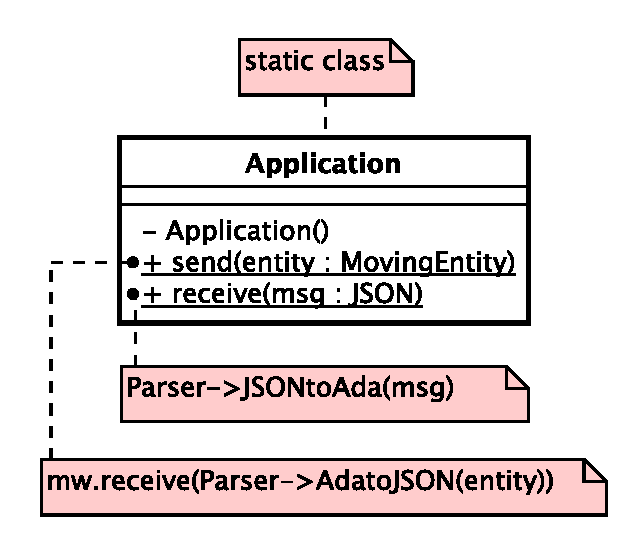
\includegraphics[scale=0.6,keepaspectratio]{images/solution/application.eps}
\caption{App::Interface::Application}
\label{fig:sd-app-application}
\end{figure}
\FloatBarrier
\begin{itemize}
  \item \textbf{Description} \\
    Lightweight interface to communicate with the middleware layer.
  \item \textbf{Attribute}
  \begin{itemize}
    \item \texttt{- parser: Parser} \\
The parser object used to convert JSON data to Ada instructions and vice versa.
  \end{itemize}
  \item \textbf{Operation}
  \begin{itemize} 
    \item \texttt{+ send(entity: MovingEntity)} \\
Sends messages to the middleware layer. Before sending the message to the
middleware it converts the entity into a JSON message using the parser.
    \item \texttt{+ receive(msg: JSON)} \\
Receives a JSON messae from the middleware layer. It invokes the parser 
passing the message as parameter.
  \end{itemize}
\end{itemize}
